% M.ahmadi 1395.11.28
% دو بار پردازش با زی‌لاتک
\PassOptionsToPackage{pdfpagemode=FullScreen,hyperfootnotes=false}{hyperref}
\documentclass[10pt,xcolor=dvipsnames,professionalfont]{beamer}

\usepackage{amsmath,amssymb,amsfonts} 
\usepackage{tikz} 
\usepackage{graphicx}
\usepackage{listings}
\usepackage{ptext}

\usetheme{Warsaw}
\usefonttheme{serif}
\usecolortheme[named=blue]{structure}
\setbeamercovered{transparent}


%% برای قرار گرفتن شماره اسلاید
\expandafter\def\expandafter\insertshorttitle\expandafter{%
\insertshorttitle\hfill%
\inserttotalframenumber\,/\,\insertframenumber}
 %%%%%%%%%%%%%%
 %توجه: بسته هایی که نیاز هست قبل از بسته زی‌پرشین نوشته شود.
\usepackage{xepersian}
\settextfont{XB Zar}
\setlatintextfont{Times New Roman}
\setdigitfont{Yas}

\defpersianfont\nas[Scale=1.5]{IranNastaliq}
\defpersianfont\xb[Scale=1.3]{XB Zar}

\deflatinfont\tnr[Scale=1.2]{Times New Roman}
%\linespread{1.2} 

%%%%%%%%%%%%%%%
\definecolor{mygreen}{RGB}{28,172,0} 
\definecolor{mylilas}{RGB}{170,55,241}
\lstset{language=Matlab,
    breaklines=true,basicstyle=\ttfamily\scriptsize,
    morekeywords={matlab2tikz},
    keywordstyle=\color{blue},
    morekeywords=[2]{1}, keywordstyle=[2]{\color{black}},
    identifierstyle=\color{black},
    stringstyle=\color{mylilas},
    commentstyle=\color{mygreen},
    showstringspaces=false
}

% دستورات مورد نیاز برای استفاده از کلاس بیمر در command نوشته شده
%
% M.ahmadi 1395.11.08, copy of:
% http://qa.parsilatex.com/14100
% http://qa.parsilatex.com/14148
%%%%%%%%%%%%%%%%%
\makeatletter
\define@key{beamercolbox}{left}[0pt]{\def\beamer@colbox@rs{0pt}\def\beamer@colbox@ls{#1 plus1fill}}
\makeatother
%%%%%%%%%%%%%%%%%
\makeatletter
\expandafter\let\csname beamer@@tmpop@itemize item@default\endcsname\relax
\expandafter\let\csname beamer@@tmpop@itemize subitem@default\endcsname\relax
\expandafter\let\csname beamer@@tmpop@itemize subsubitem@default\endcsname\relax

\defbeamertemplate*{itemize item}{default}{\scriptsize\raise1.25pt\hbox{\donotcoloroutermaths$\blacktriangleleft$}}
\defbeamertemplate*{itemize subitem}{default}{\tiny\raise1.5pt\hbox{\donotcoloroutermaths$\blacktriangleleft$}}
\defbeamertemplate*{itemize subsubitem}{default}{\tiny\raise1.5pt\hbox{\donotcoloroutermaths$\blacktriangleleft$}}

\bidi@patchcmd{\@listi}{\leftmargin}{\rightmargin}{}{}
\let\@listI\@listi
\bidi@patchcmd{\@listii}{\leftmargin}{\rightmargin}{}{}
\bidi@patchcmd{\@listiii}{\leftmargin}{\rightmargin}{}{}
\bidi@patchcmd{\beamer@enum@}{\raggedright}{\raggedleft}{}{}
\bidi@patchcmd{\@@description}{\raggedright}{\raggedleft}{}{}
\bidi@patchcmd{\@@description}{\leftmargin}{\rightmargin}{}{}

\renewcommand{\itemize}[1][]{%
  \beamer@ifempty{#1}{}{\def\beamer@defaultospec{#1}}%
  \ifnum \@itemdepth >2\relax\@toodeep\else
    \advance\@itemdepth\@ne
    \beamer@computepref\@itemdepth% sets \beameritemnestingprefix
    \usebeamerfont{itemize/enumerate \beameritemnestingprefix body}%
    \usebeamercolor[fg]{itemize/enumerate \beameritemnestingprefix body}%
    \usebeamertemplate{itemize/enumerate \beameritemnestingprefix body begin}%
    \list
      {\usebeamertemplate{itemize \beameritemnestingprefix item}}
      {\def\makelabel##1{%
          {%
            \hss\llap{{%
                \usebeamerfont*{itemize \beameritemnestingprefix item}%
                \usebeamercolor[fg]{itemize \beameritemnestingprefix item}##1}}%
          }%
        }%
      }
  \fi%
  \beamer@cramped%
  \raggedleft%
  \beamer@firstlineitemizeunskip%
}
\makeatother
%%%%%%%%%%%%%%%%%
\makeatletter
\bidi@undef\beamer@@tmpop@footnote@default

\defbeamertemplate*{footnote}{default}
{
  \parindent 1em\noindent%
  \raggedleft
  \hbox to 1.8em{\hfil\insertfootnotemark}\insertfootnotetext\par%
}

\defbeamertemplate*{LTRfootnote}{default}
{
  \parindent 1em\noindent%
  \raggedright
  \hbox to 1.8em{\hfil\insertfootnotemark}\latinfont\insertfootnotetext\par%
}
\footdir@temp\footdir@ORG@bidi@beamer@framefootnotetext\beamer@framefootnotetext{R}
\let\@footnotetext=\beamer@framefootnotetext
\let\@RTLfootnotetext\@footnotetext

\def\@makeLTRfntext#1{%
  \def\insertfootnotetext{#1}%
  \def\insertfootnotemark{\@makefnmark}%
  \usebeamertemplate***{LTRfootnote}}

\newcommand<>\beamer@frameLTRfootnotetext[1]{%
  \global\setbox\beamer@footins\vbox{\@RTLfalse%
    \hsize\framewidth
    \textwidth\hsize
    \columnwidth\hsize
    \unvbox\beamer@footins
    \reset@font\footnotesize
    \@parboxrestore
    \protected@edef\@currentlabel
         {\csname p@footnote\endcsname\@thefnmark}%
    \color@begingroup
      \uncover#2{\@makeLTRfntext{%
        \rule\z@\footnotesep\ignorespaces#1\@finalstrut\strutbox}}%
    \color@endgroup}}


\footdir@temp\footdir@ORG@bidi@beamer@frameLTRfootnotetext\beamer@frameLTRfootnotetext{L}
\let\@LTRfootnotetext=\beamer@frameLTRfootnotetext

\makeatother
%%%%%%%%%%%%%%
\makeatletter
\renewenvironment{beamercolorbox}[2][]{%
  \begingroup%
    \def\beamer@colbox@coladd{0pt}%
    \def\beamer@vmode{\leavevmode}%
    \setkeys{beamercolbox}{%
      wd=\textwidth,ht={},dp={},%
      rightskip=0pt,leftskip=0pt plus1fil,%
      sep=0pt,colsep=0pt,colsep*=0pt,%
      shadow=false,rounded=false,ignorebg=false}%
    \setkeys{beamercolbox}{#1}%
    \ifbeamercolorempty[bg]{#2}{\@tempswafalse}{\@tempswatrue}%
    \ifbeamer@colbox@ignorebg\@tempswafalse\fi%
    \def\beamer@colbox@color{#2}%
    \hsize=\beamer@colbox@wd%
    \setbox\beamer@tempbox=\hbox\bgroup\vbox\bgroup%
      \leftskip=\beamer@colbox@ls%
      \advance\leftskip by\beamer@colbox@sep%
      \rightskip=\beamer@colbox@rs%
      \advance\rightskip by\beamer@colbox@sep%
      \ifbeamer@colbox@ignorebg%
        \colorlet{beamer@temp@color}{bg}%
        \usebeamercolor[fg]{#2}%
        \colorlet{bg}{beamer@temp@color}%
      \else%
        \usebeamercolor[fg]{#2}%
      \fi%
      \if@tempswa%
        \advance\leftskip by\beamer@colbox@colsep%
        \advance\rightskip by\beamer@colbox@colsep%
        \ifdim\beamer@colbox@colsep=0pt\else\vskip\beamer@colbox@colsep\fi%
        \ifdim\beamer@colbox@colseps=0pt\else\vskip\beamer@colbox@colseps\fi%
      \fi%
      \ifdim\beamer@colbox@sep=0pt\else\vskip\beamer@colbox@sep\fi%
      \beamer@vmode\ignorespaces}{%
      \ifdim\beamer@colbox@sep=0pt\else\vskip\beamer@colbox@sep\fi%
      \if@tempswa\ifdim\beamer@colbox@colsep=0pt\else\vskip\beamer@colbox@colsep\fi\fi%
      \if@tempswa\ifdim\beamer@colbox@colseps=0pt\else\vskip\beamer@colbox@colseps\fi\fi%
    \egroup\egroup%
    \wd\beamer@tempbox=\hsize%
    \@tempdima=\wd\beamer@tempbox%
    \ifx\beamer@colbox@ht\@empty%
    \else%
      \ht\beamer@tempbox=\beamer@colbox@ht%
    \fi%
    \ifx\beamer@colbox@dp\@empty%
    \else%
      \dp\beamer@tempbox=\beamer@colbox@dp%
    \fi%
    \ifbeamer@colbox@rounded%
      \if@tempswa%
        \begin{beamerboxesrounded}[%
          shadow=\beamer@colbox@shadow,%
          lower=\beamer@colbox@color,%
          upper=normal text,%
          width=\beamer@colbox@wd]{}%
          \box\beamer@tempbox%
        \end{beamerboxesrounded}%
      \else%
        \ifdim\@tempdima>\textwidth%
          \setbox\beamer@tempbox=\hbox to\textwidth{\hss\box\beamer@tempbox\hss}%
        \fi%
        \box\beamer@tempbox%
      \fi%
    \else%
      \if@tempswa\setbox\beamer@tempbox=\hbox{\vbox{%
        \usebeamercolor{\beamer@colbox@color}%
        \advance\hsize by \beamer@colbox@colseps\relax%
        \advance\hsize by \beamer@colbox@colseps\relax%
        \hskip-\beamer@colbox@colseps%
        \fboxsep=0pt\colorbox{bg}{%
          \hskip\beamer@colbox@colseps%
          \hbox{\box\beamer@tempbox}%
          \hskip\beamer@colbox@colseps%
        }%
        \hskip-\beamer@colbox@colseps%
      }}\fi%
      \ifdim\@tempdima>\textwidth%
        \setbox\beamer@tempbox=\hbox to\textwidth{\hskip0pt minus\beamer@leftmargin\relax\box\beamer@tempbox\hskip0pt minus\beamer@rightmargin\relax}%
      \fi%
      \box\beamer@tempbox%
    \fi%
  \endgroup%
}
\makeatother
%%%%%%%%%%%%%%%%%%%%%%%
\makeatletter
\long\def\beamer@newenvnoopt#1#2#3#4{%
  \expandafter\renewcommand\expandafter<\expandafter>\csname#1\endcsname[#2]{#3}%<- here
  \expandafter\long\expandafter\def\csname end#1\endcsname{#4}%
}
\long\def\beamer@newenvopt#1#2[#3]#4#5{%
  \expandafter\renewcommand\expandafter<\expandafter>\csname#1\endcsname[#2][#3]{#4}%<- here
  \expandafter\long\expandafter\def\csname end#1\endcsname{#5}%
}

\renewcommand<>\beamer@columncom[2][\beamer@colmode]{%
  \beamer@colclose%
  \def\beamer@colclose{\end{minipage}\hfill\end{actionenv}\ignorespaces}%
\begin{actionenv}#3%
  \setkeys{beamer@col}{#1}%
  \begin{minipage}[\beamer@colalign]{#2}%
    \leavevmode\raggedleft\beamer@colheadskip\ignorespaces}

\renewenvironment<>{columns}[1][]{%
  \begin{actionenv}#2%
  \def\beamer@colentrycode{%
    \hbox to\textwidth\bgroup%
    \leavevmode%
    \hskip-\beamer@leftmargin%
    \nobreak%
    \beamer@tempdim=\textwidth%
    \advance\beamer@tempdim by\beamer@leftmargin%
    \advance\beamer@tempdim by\beamer@rightmargin%
    \hbox to\beamer@tempdim\bgroup%
    \hbox{}\hfill\ignorespaces}%
  \def\beamer@colexitcode{\egroup%
    \nobreak%
    \hskip-\beamer@rightmargin\egroup}%
  \ifbeamer@centered\setkeys{beamer@col}{c}\else\setkeys{beamer@col}{t}\fi%
  \setkeys{beamer@col}{#1}%
  \par%
  \leavevmode\beamer@colentrycode%
  \def\beamer@colclose{}\ignorespaces}%
  {\beamer@colclose\def\beamer@colclose{}\beamer@colexitcode\end{actionenv}}%

\makeatother
%%%%%%%%%%%%%%%%%%%%%%%%%%%
\makeatletter
\expandafter\let\csname beamer@@tmpop@subsection in toc@default\endcsname\relax
\expandafter\let\csname beamer@@tmpop@subsubsection in toc@default\endcsname\relax
\defbeamertemplate*{subsection in toc}{default}
{\leavevmode\rightskip=1.5em\inserttocsubsection\par}

\defbeamertemplate*{subsubsection in toc}{default}
{\leavevmode\normalsize\usebeamerfont{subsection in toc}\rightskip=3em%
  \usebeamerfont{subsubsection in toc}\inserttocsubsubsection\par}
\makeatother
%%%%%%%%%%%%%%%%
\makeatletter
\expandafter\let\csname beamer@@tmpop@frametitle@shadow theme\endcsname\relax

\defbeamertemplate*{frametitle}{shadow theme}
{%
  \nointerlineskip%
  \vskip-2pt%
  \hbox{\leavevmode
    \advance\beamer@leftmargin by -12bp%
    \advance\beamer@rightmargin by -12bp%
    \beamer@tempdim=\textwidth%
    \advance\beamer@tempdim by \beamer@leftmargin%
    \advance\beamer@tempdim by \beamer@rightmargin%
    \hskip-\Gm@lmargin\hbox{%
      \setbox\beamer@tempbox=\hbox{\begin{minipage}[b]{\paperwidth}%
          \vbox{}\vskip-.75ex%
          \rightskip0.3cm
          \leftskip0.3cm plus1fil\leavevmode
          \insertframetitle%
          \ifx\insertframesubtitle\@empty%
            \strut\par%
          \else
            \par{\usebeamerfont*{framesubtitle}{\usebeamercolor[fg]{framesubtitle}\insertframesubtitle}\strut\par}%
          \fi%
          \nointerlineskip
          \vbox{}%
          \end{minipage}}%
      \beamer@tempdim=\ht\beamer@tempbox%
      \advance\beamer@tempdim by 2pt%
      \begin{pgfpicture}{0pt}{0pt}{\paperwidth}{\beamer@tempdim}
        \usebeamercolor{frametitle right}
        \pgfpathrectangle{\pgfpointorigin}{\pgfpoint{\paperwidth}{\beamer@tempdim}}
        \pgfusepath{clip}
        \pgftext[left,base]{\pgfuseshading{beamer@frametitleshade}}
      \end{pgfpicture}
      \hskip-\paperwidth%
      \box\beamer@tempbox%
    }%
    \hskip-\Gm@rmargin%
  }%
  \nointerlineskip
    \vskip-0.2pt
    \hbox to\textwidth{\hskip-\Gm@lmargin\pgfuseshading{beamer@topshade}\hskip-\Gm@rmargin}
    \vskip-2pt
}
\makeatother

%%%%%%%%%%%%%%%%%%
%http://qa.parsilatex.com/23902
\makeatletter
\expandafter\let\csname beamer@@tmpop@section in toc@ball\endcsname\relax
\defbeamertemplate{section in toc}{ball}
{\leavevmode\rightskip=2.75ex%
  \llap{%
    \normalsize%
    \begin{pgfpicture}{-1ex}{-0.7ex}{1ex}{1ex}
      \pgftext{\beamer@usesphere{section number projected}{tocsphere}}
      \pgftext{%
        \usebeamerfont*{section number projected}%
        \usebeamercolor{section number projected}%
        \color{fg!90!bg}%
        \inserttocsectionnumber}
    \end{pgfpicture}%
    \kern1.25ex}%
  \inserttocsection\par
}
[action]
{\setbeamerfont{section number projected}{size=\scriptsize}}
\expandafter\let\csname beamer@@tmpop@subsection in toc@ball\endcsname\relax
\defbeamertemplate{subsection in toc}{ball}
{\leavevmode\rightskip=5ex%
  \llap{\raise0.1ex\beamer@usesphere{subsection number projected}{bigsphere}\kern1ex}%
  \inserttocsubsection\par%
}
\expandafter\let\csname beamer@@tmpop@subsubsection in toc@ball\endcsname\relax
\defbeamertemplate{subsubsection in toc}{ball}
{\leavevmode\normalsize\usebeamerfont{subsection in
    toc}\rightskip=7ex\usebeamerfont{subsubsection in toc}%
  \llap{\beamer@usesphere{subsubsection number projected}{bigsphere}\kern0.75ex}%
  \inserttocsubsubsection\par%
}
\setbeamertemplate{sections/subsections in toc}[ball]
\makeatother


\raggedleft
%%%%%%%%%%%%%%%%%%
\newcommand*{\co}[1]{\nas\textcolor{blue}{#1}}

\title{ساخت مدل و آموزش آن به وسیله \lr{Keras}}
\author[علیرضا بیکی]{\co{علیرضا بیکی}
}
\institute{دانشگاه شیراز}
\date{\today}

\logo{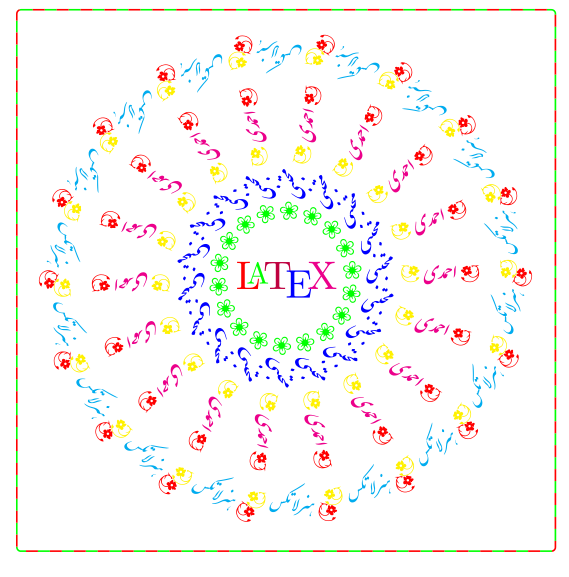
\includegraphics[scale=.04]{logo1.png} }
\newcommand{\nologo}{\setbeamertemplate{logo}{}}
%%%%%%%%%%%%%
%برای شماره خوردن قضیه،...
\setbeamertemplate{theorems}[numbered]
%بولد
\providetranslation{Theorem}{\large \bf قضیه}
\providetranslation{Definition}{تعریف}
\providetranslation{Example}{مثال}


\begin{document}

\begin{frame}
\maketitle
\end{frame}

\begin{frame}{فهرست مطالب}
\tableofcontents
\end{frame}


\section{ساخت مدل}


\begin{frame}
برای ساخت مدل در \lr{Keras} می‌توان از دو روش استفاده کرد:
\begin{enumerate}
\item
\lr{Sequential}: 
در این حالت یک مدل \lr{Sequential} درست می‌کنیم و به ترتیب لایه‌ها را به مدل اضافه می‌کنیم.
\item
\lr{Functional API}: 
در این روش ما لایه‌ها را به دلخواه خود می‌سازیم سپس این لایه‌ها را در مسیری که باید تبدیل به مدل شود را ایجاد می‌کنیم. از مزیت‌های این روش این است که می‌توانیم مدل‌های غیرمرسوم مانند مدل‌هایی که چند ورودی یا چند خروجی دارند، مثل مدل \lr{Unet}، را تولید کنیم. 
\end{enumerate}

\end{frame}

\subsection{ساخت مدل \lr{Sequential} در \lr{Keras}}
\begin{frame}[fragile]{ساخت مدل \lr{Sequential} در \lr{Keras}}
ابتدا با دستور زیر مدل \lr{Sequential} را وارد می‌کنیم:
\begin{latin}
\begin{lstlisting}[language=Python,frame=single,rulecolor=\color{magenta},numbers=left,numberstyle=\tiny]
from keras.model import Sequential
\end{lstlisting}
\end{latin}

حال باید لایه‌های مورد نظر خود (مانند لایه‌های \lr{FC, CNN, RNN,  ...}) را ایجاد کنیم. برای این منظور لایه‌ مورد نظر را با دستور زیر وارد می‌کنیم:
\begin{latin}
\begin{lstlisting}[language=Python,frame=single,rulecolor=\color{magenta},numbers=left,numberstyle=\tiny]
from keras.layers import Dense
\end{lstlisting}
\end{latin}

\begin{block}{توجه}
لایه‌های \lr{Fully Connected} در \lr{Keras} تحت عنوان لایه‌های \lr{Dense} شناخته می‌شود.
\end{block}

\end{frame}


\begin{frame}[fragile]
حال مدل را با دستور زیر ایجاد می‌کنیم:
\begin{latin}
\begin{lstlisting}[language=Python,frame=single,rulecolor=\color{magenta},numbers=left,numberstyle=\tiny]
modelName=Sequential()
\end{lstlisting}
\end{latin}
حالا لایه‌های مورد نظر را با دستور زیر اضافه می‌کنیم:
\begin{latin}
\begin{lstlisting}[language=Python,frame=single,rulecolor=\color{magenta},numbers=left,numberstyle=\tiny]
modelName.add(Dense(500, activation='relu', input_shape=(784,1)))
\end{lstlisting}
\end{latin}

\begin{itemize}
\item
پارامتر اول (500) بیانگر تعداد نورون‌های ورودی را می‌خواهد.
\vspace{0.5cm}

\item
پارامتر دوم، تابع \lr{activation} می‌باشد که به صورت پیش‌فرض مقدار \lr{None} دارد. برای مقداردهی به آن به 2 طریق می‌توان اقدام کرد:
\begin{center}
\begin{itemize}
\item[-]
همانند آنچه در بالا نشان داده شده است می‌توان نام تابع \lr{activation} را بین ` ` آورد.
\item[-]
تابع \lr{activation} را وارد کنیم و سپس نام آن را بدون ` ` بنویسیم.
\end{itemize}
\end{center}

\begin{latin}
\begin{lstlisting}[language=Python,frame=single,rulecolor=\color{magenta},numbers=left,numberstyle=\tiny]
from keras.activations import relu
modelName.add(Dense(500, activation=relu, input_shape=(784,1)))
\end{lstlisting}
\end{latin}

\end{itemize}

\end{frame}


\begin{frame}[fragile]

\begin{latin}
\begin{lstlisting}[language=Python,frame=single,rulecolor=\color{magenta},numbers=left,numberstyle=\tiny]
modelName.add(Dense(500, activation='relu', input_shape=(784,1)))
\end{lstlisting}
\end{latin}

\begin{itemize}
\item
پارامتر سوم تعداد نورون‌هایی هست که وارد لایه اول می‌شود ($784, 1$).
\end{itemize}

\begin{block}{نکته}
این کار فقط برای لایه اول لازم است و برای لایه‌های بعدی نیاز نیست.
\end{block}
به‌طور مشابه می‌توان لایه‌های بعدی را نیز تولید کرد:
\begin{latin}
\begin{lstlisting}[language=Python,frame=single,rulecolor=\color{magenta},numbers=left,numberstyle=\tiny]
modelName.add(Dense(500, activation='relu'))
modelName.add(Dense(10, activation='softmax'))
\end{lstlisting}
\end{latin}

\begin{block}{نکته}
معمولاً در خروجی از \lr{softmax} برای \lr{activation} استفاده می‌کنند.
\end{block}

\end{frame}

\subsection{ساخت مدل با \lr{Functional API} در \lr{Keras}}

\begin{frame}[fragile]{ساخت مدل با \lr{Functional API} در \lr{Keras}}


\end{frame}

\subsection{نکات تکمیلی}

\begin{frame}[fragile]{نکات تکمیلی}
با استفاده از دستور زیر می‌توان اطلاعات مختصری از مدل را نمایش داد:
\begin{latin}
\begin{lstlisting}[language=Python,frame=single,rulecolor=\color{magenta},numbers=left,numberstyle=\tiny]
modelName.summary()
\end{lstlisting}
\end{latin}
وقتی که مدل را ساختیم، باز هم می‌توانیم به لایه‌های مدل دسترسی داشته باشیم و یا تغییراتی بر روی آن‌ها انجام دهیم.
\begin{itemize}
\item
اگر بخواهیم نام لایه را تغییر بدهیم (لایه اول، برابر صفر است):
\begin{latin}
\begin{lstlisting}[language=Python,frame=single,rulecolor=\color{magenta},numbers=left,numberstyle=\tiny]
modelName.layers[0]='layer_0'
\end{lstlisting}
\end{latin}
\item
اگر بخواهیم لایه صفر در بحث آموزش شرکت نکند:
\begin{latin}
\begin{lstlisting}[language=Python,frame=single,rulecolor=\color{magenta},numbers=left,numberstyle=\tiny]
modelName.layers[0].trainable=False
\end{lstlisting}
\end{latin}

\item
تمام پارامترهای یک لایه را که ما می‌توانیم ببینیم یا تغییری بر رو آن‌ها انجام دهیم، به ما می‌‌دهد.
\begin{latin}
\begin{lstlisting}[language=Python,frame=single,rulecolor=\color{magenta},numbers=left,numberstyle=\tiny]
modelName.layers[0].get_config()
\end{lstlisting}
\end{latin}
\end{itemize}

\end{frame}


\section{کامپایل کردن مدل}
\begin{frame}[fragile]{کامپایل کردن مدل}
آخرین مرحله از ساختن مدل این است که مدل را کامپایل کنیم و پارامترهایی که مدل نیاز دارد با به آن بدهیم.
\begin{latin}
\begin{lstlisting}[language=Python,frame=single,rulecolor=\color{magenta},numbers=left,numberstyle=\tiny]
modelName.compile(optimizer='SGD', loss=categorical_crossentropy, metric=[`accuracy`])
\end{lstlisting}
\end{latin}

\begin{itemize}
\item
پارامتر اول تابع بهینه‌ساز می‌باشد که این نیز می‌تواند به 2 صورت استفاده شود:
\begin{itemize}
\item[-]
همانند مثال، نام تابع بهینه‌سازی بین ` ` آورده شود.
\item[-]
تابع بهینه‌ساز وارد \lr{Keras} شود و بدون ` ` مورد استفاده قرار گیرد.
\end{itemize}
\end{itemize}
\vspace{-0.5cm}

\begin{latin}
\begin{lstlisting}[language=Python,frame=single,rulecolor=\color{magenta},numbers=left,numberstyle=\tiny]
from keras.optimizer import SGD
modelName.compile(optimizer=SGD(lr=0.001), loss=categorical_crossentropy, metric=[`accuracy`])
\end{lstlisting}
\end{latin}

\begin{block}{نکته}
تابع بهینه‌ساز خودش نیز دارای پارامترهای مانند \lr{Momentum}، \lr{learning rate}، \lr{decay} و \lr{nestrov} می‌باشد.
\end{block}

\end{frame}

\begin{frame}[fragile]{کامپایل کردن مدل}
\begin{latin}
\begin{lstlisting}[language=Python,frame=single,rulecolor=\color{magenta},numbers=left,numberstyle=\tiny]
modelName.compile(optimizer='SGD', loss=categorical_crossentropy, metric=[`accuracy`])
\end{lstlisting}
\end{latin}
\begin{itemize}
\item
پارامتر دوم تابع \lr{loss} می‌باشد که به صورت زیر وارد \lr{keras} می‌کنیم:
\begin{latin}
\begin{lstlisting}[language=Python,frame=single,rulecolor=\color{magenta},numbers=left,numberstyle=\tiny]
from keras.layers import categorical_crossentropy
\end{lstlisting}
\end{latin}
\item
در پارامتر سوم \lr{accuracy} به عنوان معیار نمایش دقت مدل به کار می‌رود.
\end{itemize}

\end{frame}

\section{آموزش مدل}
\begin{frame}[fragile]{آموزش مدل}
برای آموزش مدل کافی است که از دستور \lr{fit} استفاده کنیم.
\begin{latin}
\begin{lstlisting}[language=Python,frame=single,rulecolor=\color{magenta},numbers=left,numberstyle=\tiny]
network_history=modelName.fit(x_train, y_train, batch_size=128, epoches=2, validation_split=0.2)
\end{lstlisting}
\end{latin}
\vspace{-0.3cm}
\begin{block}{نکته}
برای اینکه بتوانیم پارامترهای آموزش را بررسی کنیم، آن‌ها را درون یک متغیر به نام \lr{network\_history} قرار می‌دهیم.
\end{block}
\begin{itemize}
\item
\lr{x\_train} ورودی
\item
\lr{y\_train} خروجی مورد نظر که ورودی ما باید با آن مقایسه شود.
\item
\lr{batch\_size} تعداد داده‌هایی که در هر دوره آموزش وارد می‌شوند.
\item
\lr{epoches} تعداد تکرارهای آزمایش
\item
\lr{validation\_split} 20 درصد داد‌ها را برای اعتبارسنجی کنار می‌گذارد و از 80 درصد داده‌ها برای آموزش مدل استفاده می‌کند.
\end{itemize}

\end{frame}

\begin{frame}[fragile]{آموزش مدل}
حال می‌خواهیم مدل آموزش دیده را بر روی داده‌های \lr{test} استفاده کنیم. این کار را می‌توان با دستورهای \lr{evaluate} و \lr{predict} انجام دهیم:
\begin{latin}
\begin{lstlisting}[language=Python,frame=single,rulecolor=\color{magenta},numbers=left,numberstyle=\tiny]
test_loss=modelName.evaluate(x_test, y_test)
\end{lstlisting}
\end{latin}
با دستور \lr{predict} می‌توانیم داده‌های \lr{test} را به مدل بدهیم و خروجی آن را بخواهیم و ببینیم خروجی را چگونه پیش‌بینی می‌کند:
\begin{latin}
\begin{lstlisting}[language=Python,frame=single,rulecolor=\color{magenta},numbers=left,numberstyle=\tiny]
test_label=modelName.predict(x_test)
\end{lstlisting}
\end{latin}
\end{frame}


\section{لایه‌های Dropout}
\begin{frame}[fragile]{لایه‌های Dropout}
در خطا (\lr{loss}) جایی که نمودار \lr{train} شروع به کاهش کرد ولی نمودار \lr{validation} شروع به افزایش، آن نقطه‌ای است که احتمالاً دچار \lr{over fitting} شده است. تا اینجا باید \lr{epoch}ها را قطع کرد یا از تکنیک‌های همانند \lr{Dropout} استفاده کرد تا از \lr{over fitting} شدن جلوگیری کند.
\begin{latin}
\begin{lstlisting}[language=Python,frame=single,rulecolor=\color{magenta},numbers=left,numberstyle=\tiny]
from keras.models import Dropout
modelName.add(Dropout(0.2))
\end{lstlisting}
\end{latin}
این دستور به این معنی است که 20 درصد داده‌ها را از محاسبات خارج می‌کند.
\begin{block}{نکته}
لایه‌های \lr{Dropout} در شبکه‌های \lr{FC} معمولاً برای کاهش \lr{over fitting} استفاده می‌شود.
\end{block}

\begin{block}{نکته}
با استفاده از لایه‌های \lr{Dropout} مقدار خطا کمی افزایش پیدا می‌کند ولی برای جلوگیری از \lr{over fitting} لازم است.
\end{block}

\end{frame}










\end{document}
